\appendix
\section{Parametri del sistema}\label{sec:parametri-sistema}
\begin{table}[H]
  \centering
  \begin{tabular}[t]{cc}
    \toprule
    Parametro &Valore\\
    \midrule
    $m$ & $.150$Kg \\
    $M$ & $.175$Kg \\
    $L$ & $.38$m   \\
    $g$ & $9.8\frac {\text m}{\text {s}^2}$ \\
    \bottomrule
  \end{tabular}
  \caption{
    Parametri del sistema.
  }
  \label{tab:parametri-sistema}
\end{table}

\begin{table}[H]
  \centering
  \begin{tabular}[t]{cc}
    \toprule
    Parametro &Valore\\
    \midrule
    \vspace{5px}
    $Q$ & $\left(\begin{matrix}
                   &.1 &0 &0 &0 \\ &0 &.0001 &0 &0 \\ &0 &0 &1 &0 \\ &0 &0 &0 &.0001
    \end{matrix}\right)$ \\
    \vspace{5px}
    $R$ & $\left(\begin{matrix}
                   .005
    \end{matrix}\right)$ \\
    \vspace{5px}
    $K$ & $\left(\begin{matrix}
                   3.67 \\ 3.85 \\ 22.6 \\ 3.97
    \end{matrix}\right)$ \\
    \bottomrule
  \end{tabular}
  \caption{
    Parametri adimensionali del controller \textsc{lqr}. Le matrici $Q$ e $R$ sono definite da me, $K$ è stato ricavato.
  }
  \label{tab:coefficienti-lqr}
\end{table}

\begin{table}[H]
  \centering
  \begin{tabular}[t]{cc}
    \toprule
    Parametro &Valore\\
    \midrule
    $K_{px}$ & $2$ \\
    $K_{dx}$ & $1000$ \\
    $K_{p\theta} $ & $15$   \\
    $K_{d\theta}$ & $1300$ \\
    \bottomrule
  \end{tabular}
  \caption{
    Parametri adimensionali del controller \textsc{pid}, ricavati con il metodo \emph{trial-and-error}.
  }
  \label{tab:coefficienti-pid}
\end{table}

\section{Calibrazione del motore}\label{sec:calibrazione-motore}
Un motore DC è controllato variando il voltaggio $V$ in ingresso. La forza esercitata dal motore, tuttavia, non è
lineare rispetto a $V$. Per risolvere questo problema, possiamo usare la formula\cite{dcControl}:
  \begin{equation}
    \begin{aligned}[c]
      u_k = \frac {(1-a)v_k -c \text{sign} v_k + \Delta t \dot v_k} {b}
    \end{aligned}
    \label{eq:motore}
  \end{equation}

Ho ricavato i parametri $a$, $b$ e $c$ dal fit in figura \ref{fig:fit}; i valori numerici sono riportati in tabella \ref{tab:fit}.

\begin{figure}[h]
  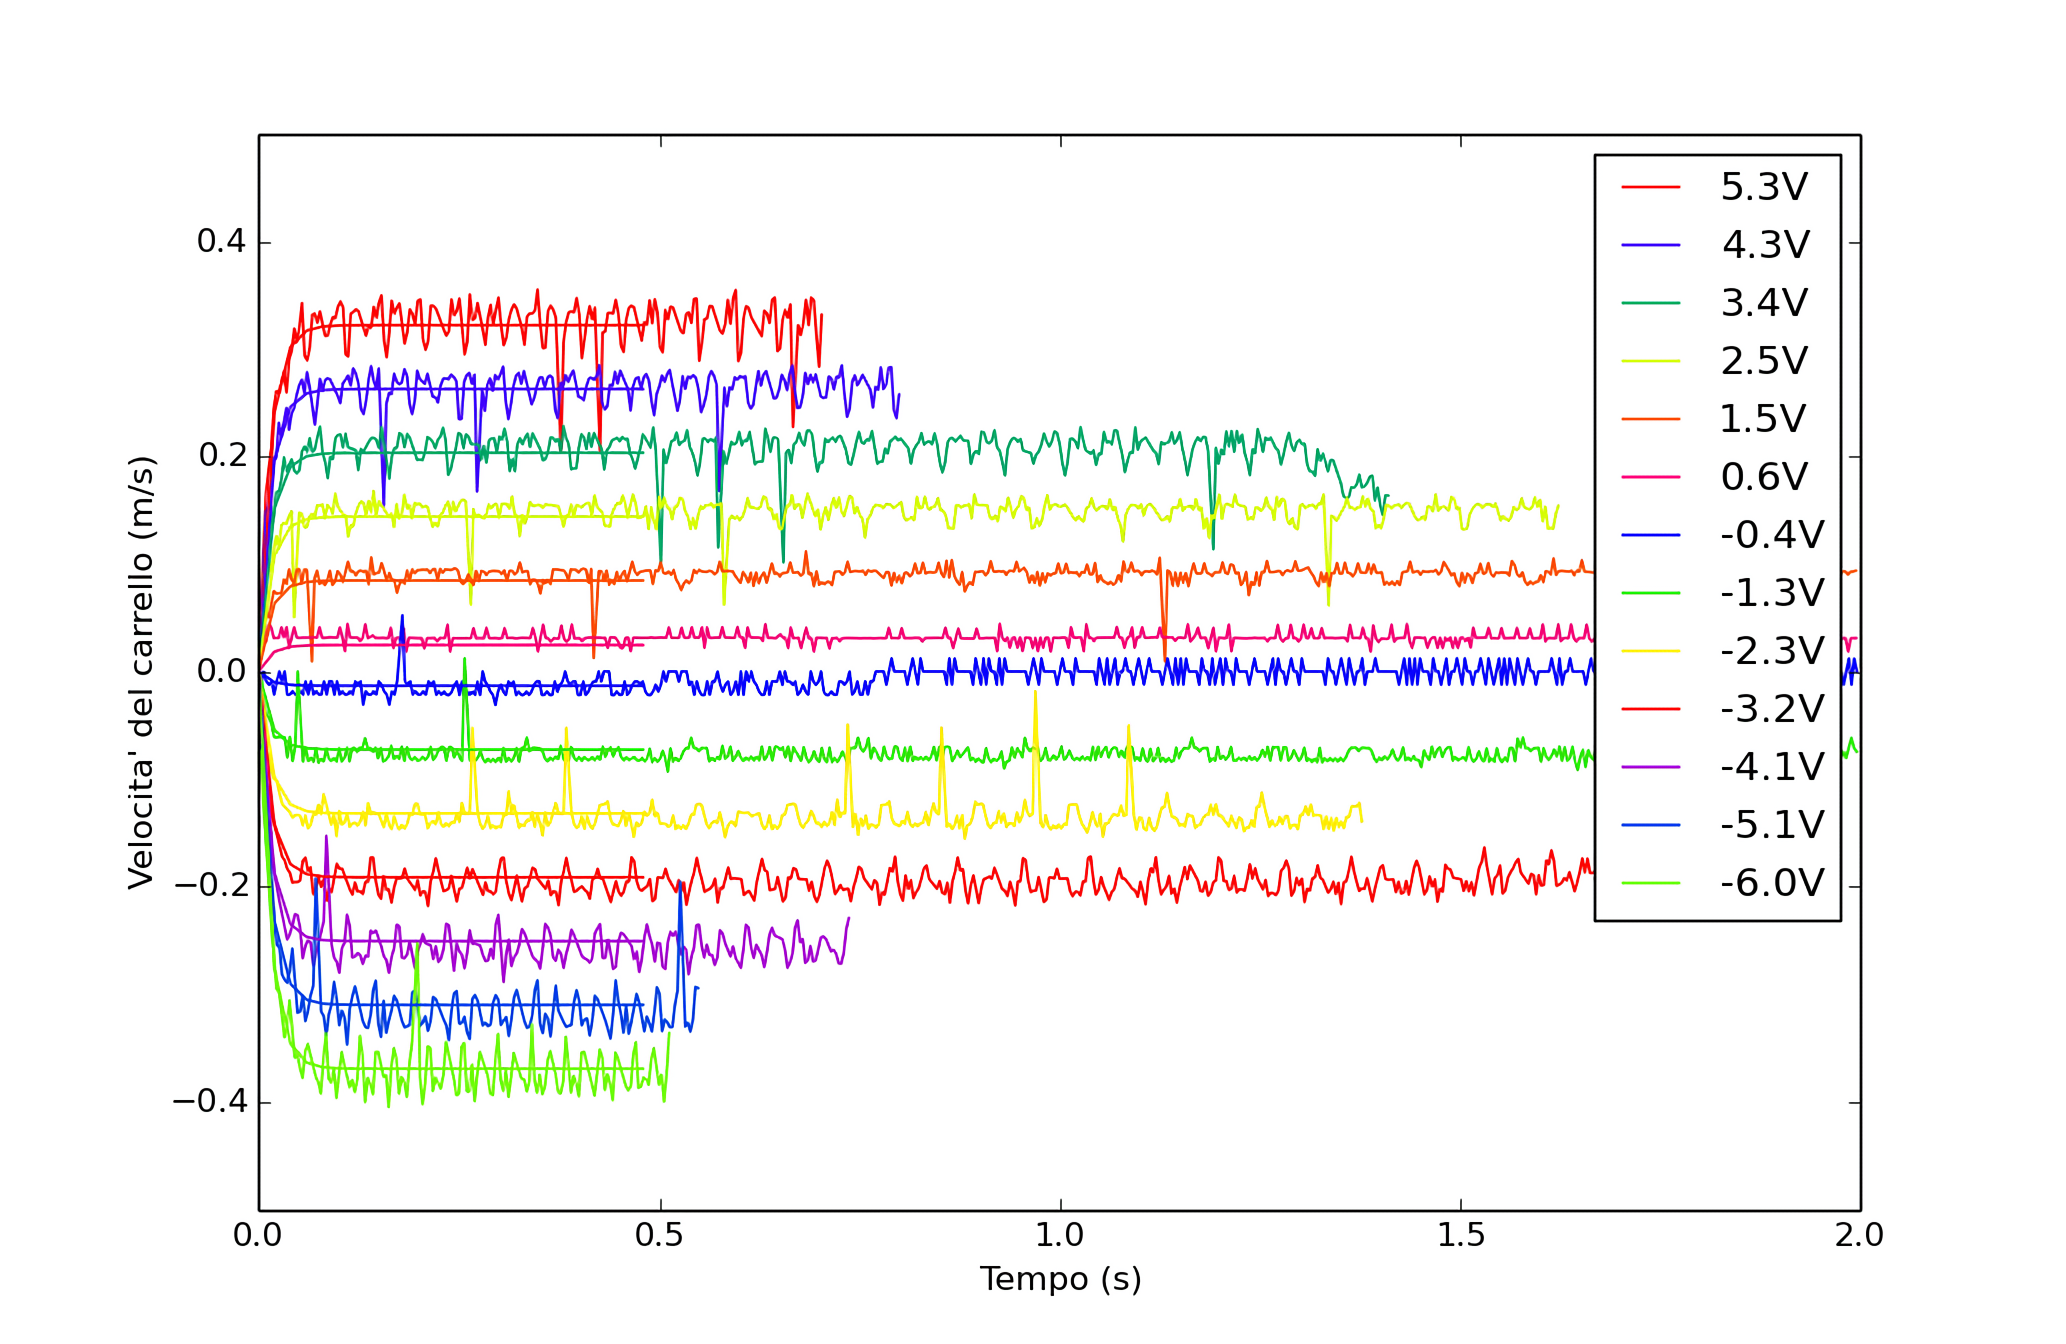
\includegraphics[width=0.47\textwidth]{../assets/fit.png} %todo cambia
  \caption{\emph{Fit dei parametri del motore.}}
  \label{fig:fit}
\end{figure}

\begin{table}[H]
  \centering
  \begin{tabular}[t]{cc}
    \toprule
    Parametro &Valore\\
    \midrule
    $a$ & $.251$ \\
    $b$ & $.047$ \\
    $c$ & $.008$ \\
    \bottomrule
  \end{tabular}
  \caption{
    Parametri adimensionali ottenuti dal fit del motore.
  }
  \label{tab:fit}
\end{table}

